\documentclass[12pt]{article}

\usepackage{tabularx}
\usepackage{booktabs}
\usepackage{fullpage}
\usepackage{graphicx}

%% Comments

\usepackage{color}

\newif\ifcomments\commentstrue %displays comments
%\newif\ifcomments\commentsfalse %so that comments do not display

\ifcomments
\newcommand{\authornote}[3]{\textcolor{#1}{[#3 ---#2]}}
\newcommand{\todo}[1]{\textcolor{red}{[TODO: #1]}}
\else
\newcommand{\authornote}[3]{}
\newcommand{\todo}[1]{}
\fi

\newcommand{\wss}[1]{\authornote{blue}{SS}{#1}} 
\newcommand{\plt}[1]{\authornote{magenta}{TPLT}{#1}} %For explanation of the template
\newcommand{\an}[1]{\authornote{cyan}{Author}{#1}}

%% Common Parts

\newcommand{\progname}{Flick Picker}
\newcommand{\authname}{Team 7, 7eam
\\ Talha Asif - asift
\\ Jarrod Colwell - colwellj
\\ Madhi Nagarajan - nagarajm
\\ Andrew Carvalino - carvalia    
\\ Ali Tabar - sahraeia
}     

\usepackage{hyperref}
    \hypersetup{colorlinks=true, linkcolor=blue, citecolor=blue, filecolor=blue,
                urlcolor=blue, unicode=false}
    \urlstyle{same}
                                


\begin{document}

\title{Software Requirements Specification for \progname: Group Show Finder} 
\author{\authname}
\date{\today}
	
\maketitle
\vspace*{\fill}
Created From: Volere, Requirements Specification Template, Edition 18


~\newpage \pagenumbering{roman}

\tableofcontents

~\newpage

\section*{Revision History}

\begin{tabularx}{\textwidth}{p{3cm}p{2cm}X}
\toprule {\bf Date} & {\bf Version} & {\bf Notes}\\
\midrule
Oct 1/22 & 0.0 & Copying Volere Template and updating sections\\
Oct 1/22 & 0.1 & Adding Sections 1, 3, 5\\
Oct 2/22 & 0.2 & Adding Section 6\\
Oct 5/22 & 0.3 & Adding Section 2\\
Oct 5/22 & 0.4 & Adding Section 7\\
Oct 5/22 & 0.5 & Adding Section 4\\
Oct 5/22 & 0.6 & Adding Section 8, 10.1, 10.6\\
\bottomrule
\end{tabularx}

~\newpage \pagenumbering{arabic}

\section{The Purpose of the Project}

\subsection{The User Business or Background of the Project Effort}
The business aims to make finding shows across groups of friends with differing preferences easier by streamlining the process from start to finish. As a quick summary, users will be able to input their preferences, make groups with their friends, and the group will get recommendations based on all their preferences. In addition, an opportunity arose in the market after COVID passed as large groups can create host gatherings for any events, one such that this application can select.

\subsection{Goals of the Project}
Goals can shift as development continues, entirely losing scope on the developers' passion for why the application started. Thus there will only be a few immediate goals to capture the passion that developers currently have and will continue to uphold in the future:
\begin{itemize}
	\item Provide a means of choosing a Movie, TV show, or Anime to watch immediately in a large friend group, which they all enjoy
	\item Users can be recommended a Movie, TV show, or Anime individually as well.
	\item Minimize the number of advertisements while using the application
\end{itemize}

\section{The Stakeholders}
\subsection{The Client}
The clients for Flick Picker are Dr. Spencer Smith and the Teaching Assistants of 4G06, who will be responsible for a few key milestones in the development process.
The client will be responsible for project approval, including, but not limited to, the approval of the general idea, scope, and complexity.
Additionally, the client will also provide feedback throughout the development on various deliverables.

\subsection{The Customer}
The customers for Flick Picker are individuals who watch movies, tv shows, or anime as an individual or a group who wish to find catered recommendations.

\subsection{Other Stakeholders}

The members of 7eam are other stakeholders falling under the categories of:
\begin{itemize}
    \item Designers and Developers
    \item Testers
    \item Systems Engineers
    \item Technology Experts
    \item System Designers
    \item Usability Experts
\end{itemize}

\subsection{The Hands-On Users of the Product}
The hands-on users of the product are the same as listed under the customer section.

\subsubsection*{Individual Watchers}
The individual watcher is a user who will simply input their preference settings and then browse the movies, tv shows, or anime that fit the preferences.
\subsubsection*{Group Watchers}
Group watchers also input their personal preferences.
Additionally, they must also create a group and add the other members.
With the group created, members can browse the movies, tv shows, or anime that best fit the combined preferences of the group.

\subsection{Personas}
N/A

\subsection{Priorities Assigned to Users}
N/A

\subsection{User Participation}
N/A

\subsection{Maintenance Users and Service Technicians}
N/A

\section{Constraints}

\subsection{Solution Constraints}
There are no specific constraints the stakeholders have asked to be on the product regarding the solution. So instead, 7eam deems it necessary to have a general form of constraint on the development of Flick Picker that is the following:
\begin{itemize}
	\item Flick Picker must have in-depth tests on any part of the application before releasing it to the users and also follow a strict and healthy software engineering process
\end{itemize}
There are no specific technological constraints. However, the technology stack must follow industry standards.

\subsection{Implementation Environment of the Current System}
The application will be deployed on a website, so the restrictions of a browser follow.

\subsection{Partner or Collaborative Applications}
N/A

\subsection{Off-the-Shelf Software}
The list of Movies, TV Shows, and Anime will be polled from two separate APIs, which is the following:
\begin{itemize}
	\item MyAnimeList for data on Anime
	\item OMDB for data on TV Shows and Movies
\end{itemize}

\subsection{Anticipated Workplace Environment}
As Flick Picker is a browser application, 7eam expects users to use the application on their desktops or phones. Thus the application must be optimized for both possible settings, relying on a responsive layout. However, the users' physical workplace has no bearing on the design, as they can use it whenever necessary. 

\subsection{Schedule Constraints}
The schedule is the same as the one Dr. Smith has provided us with

\begin{tabular}{ |p{9.7cm} l|}
	\hline
	Team Formed, Project Selected & September 19\\
	\hline
	Problem Statement, Development Plan & September 26\\
	\hline
	Requirements Document Revision 0 & October 5\\
	\hline
	Hazard Analysis 0 & October 19\\
	\hline
	V\&V Plan Revision 0 & November 2\\
	\hline
	Proof of Concept Demonstration & November 14--25\\
	\hline
	Design Document Revision 0 & January 18\\
	\hline
	Revision 0 Demonstration & February 6--February 17\\
	\hline
	V\&V Report Revision 0 & March 8\\
	\hline
	Final Demonstration (Revision 1) & March 20--March 31\\
	\hline
	EXPO Demonstration & April TBD\\
	\hline
	Final Documentation (Revision 1)\newline 
	- Problem Statement\newline
	- Development Plan\newline
	- Requirements Document\newline
	- Hazard Analysis\newline
	- Design Document\newline
	- V\&V Plan\newline
	- V\&V Report\newline
	- User's Guide\newline
	- Source Code\newline & April 5\\
	\hline
\end{tabular}

\subsection{Budget Constraints}
The expenses for this application must not exceed \$500, and there are only five developers working on 7eam.

\subsection{Enterprise Constraints}
N/A

\section{Naming Conventions and Terminology}

\subsection{Glossary of All Terms, Including Acronyms, Used by Stakeholders Involved in the Project}
\begin{itemize}
	\item BE: Back-End
	\item FE: Front-End
\end{itemize}

\section{Relevant Facts and Assumptions}

\subsection{Relevant Facts}
There is no existing solution 7eam has found that fills a similar role as selecting a Movie, TV Show or Anime based on the preferences of a group of users.


\subsection{Business Rules}
N/A

\subsection{Assumptions}
There are a few assumptions 7eam deems necessary to see regarding Flick Picker's capabilities and what it will not do:
\begin{itemize}
	\item Flick Picker will not provide a means to watch the selected show directly through the application
	\item Flick Picker will suggest the best movie, tv show, or anime for the group. This may violate the preferences of a member or multiple members of the group.
	\item The browser on which the application is used, through any device, is not deprecated
\end{itemize}

\section{The Scope of the Work}

\subsection{The Current Situation}
As Flick Picker is being built from the ground up, no existing business processes exist. However, 7eam has agreed to follow a rigorous development process, which is not changing. The developers must make a pull request against the `develop' branch to make any changes, which two people must review before merging. If it is a code change, then tests must run on the deployed code, all passing and getting two reviews before merging.

\subsection{The Context of the Work}
\begin{center}
	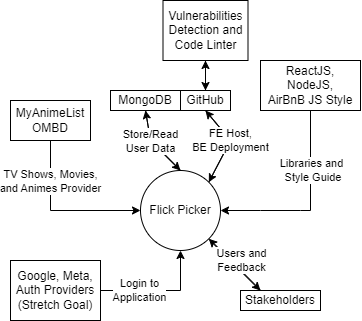
\includegraphics[scale=1]{contextDiagram.png}
\end{center}

\subsection{Work Partitioning}
\subsubsection*{Business Event List}
\begin{tabularx}{\textwidth}{|p{4cm}p{6cm}X|}
\toprule {\bf Event Name} & {\bf Input and Output} & {\bf Summary of BUC}\\
\hline
MyAnimeList/OMBD are polled & TV Show, Movie, and Anime Data (in) & Collect information about the shows to display to users \\
\hline
MongoDB data is updated & User data updated (out) & Any updates to user data are stored \\
\hline
MongoDB data is queried & User data retrieved (in) & Fetches everything needed for the user after login \\
\hline
Code is updated & GitHub redeploys new changes (in/out) & Updates the FE or BE deployment any time there is a merge to server \\
\hline
Deprecated library is used & Vulnerability detection blocks changes (in) & Deployment protection such that libraries are safe to use \\
\hline
Code does not match style & AirBnB style guide (in), Linter updates code (in/out) & Enforces the style guide on FE/BE development \\
\hline
External login is queried & External authentication validates user (in) & Allows users to log in with industry standard authentication providers \\
\hline
\end{tabularx}

\subsection{Specifying a Business Use Case (BUC)}
N/A as summary of BUCs are above.

\section{Business Data Model and Data Dictionary}
\subsection{Business Data Model}
\begin{center}
	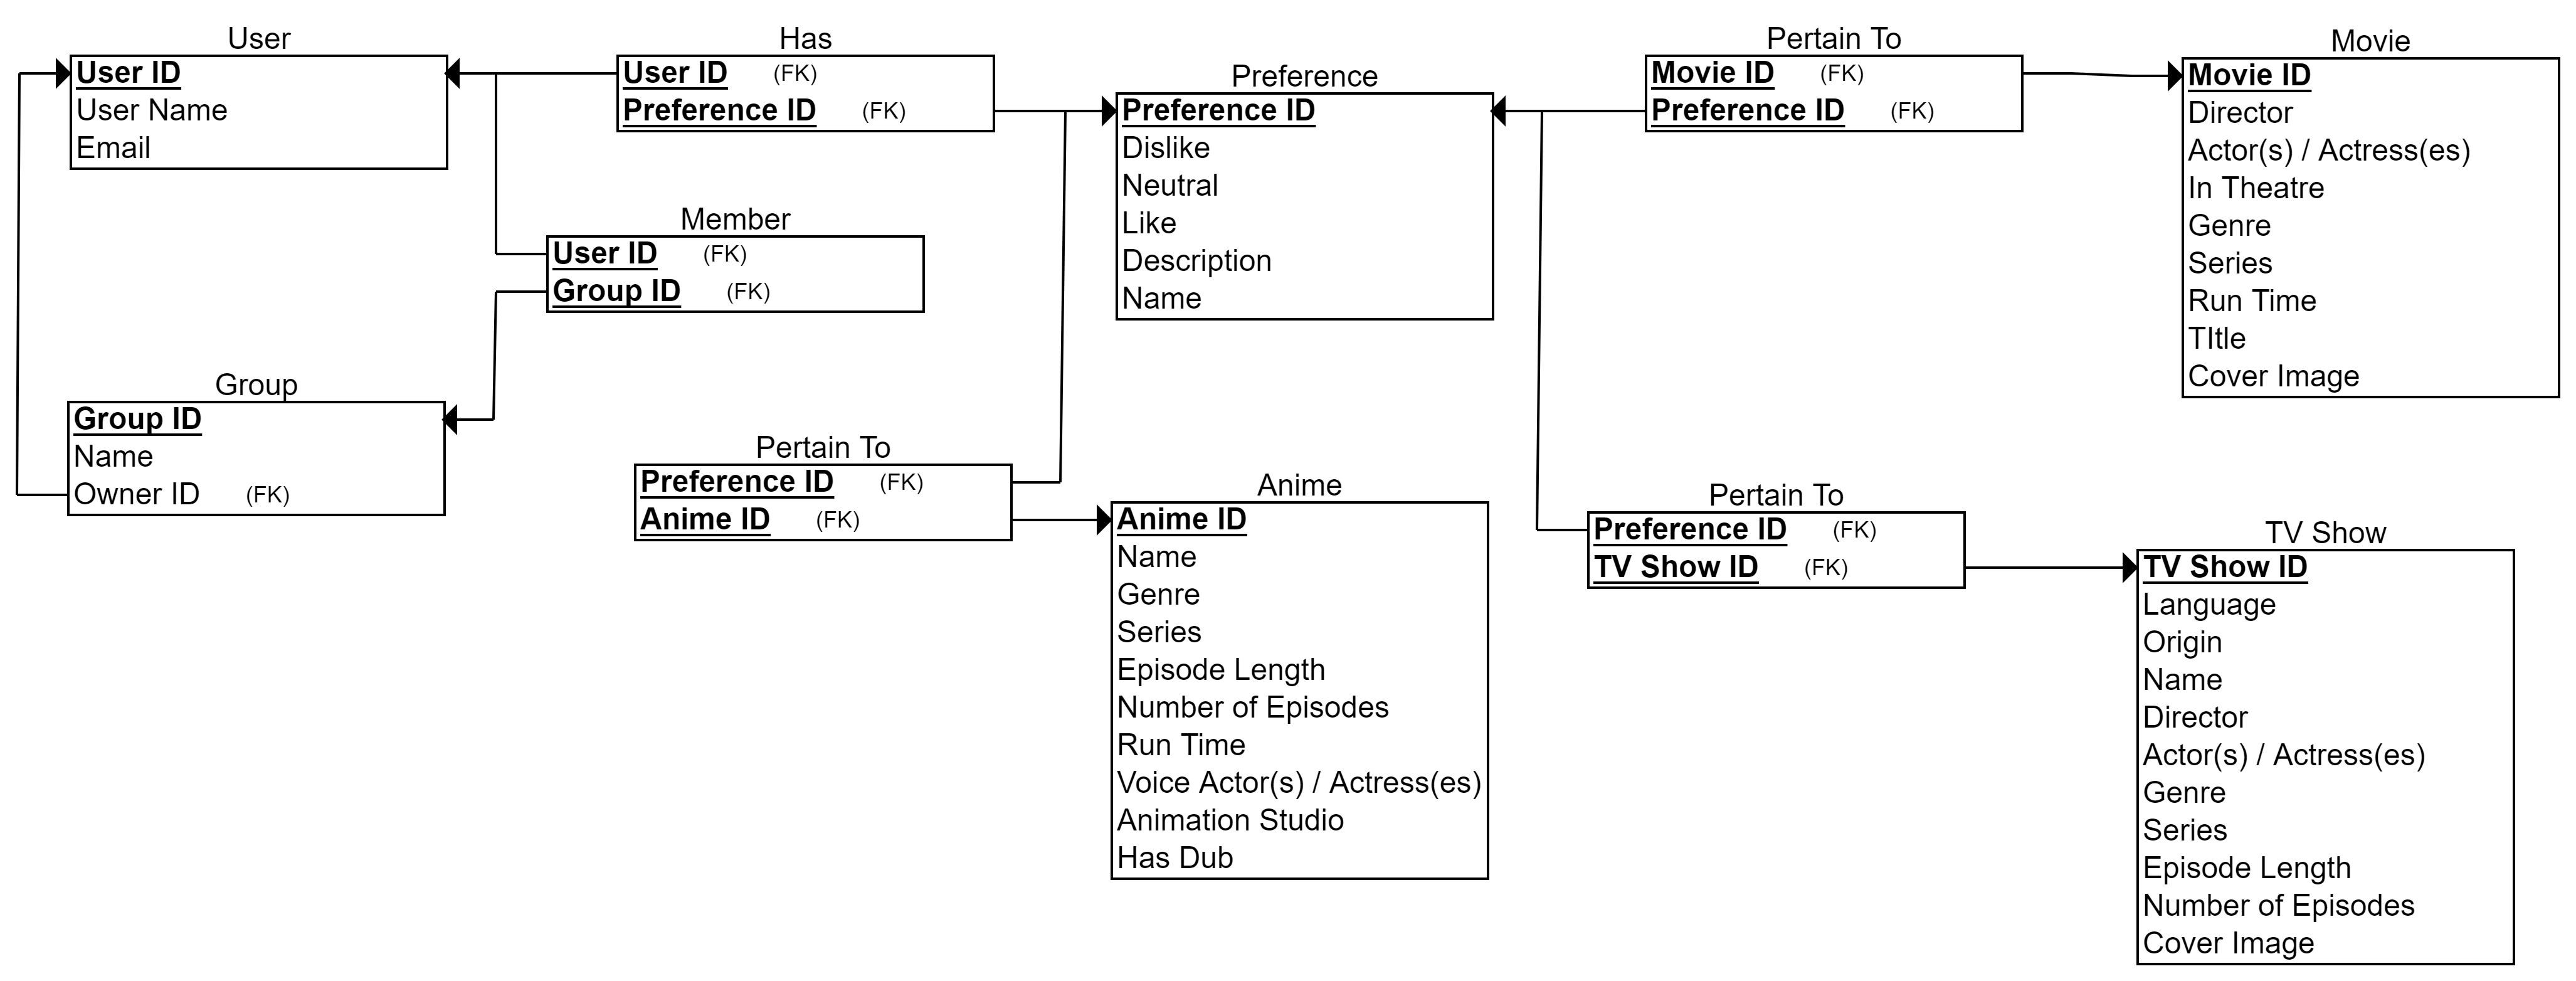
\includegraphics[scale=0.12]{BusinessDataModel.png}
\end{center}

\subsection{Data Dictionary}
For content of each element of the data dictionary, see the Business Data Model above.
Additionally, attributes that are self explanatory are omitted from the Data Dictionary for document size purposes, they are assumed to be members of the data dictionary.

\begin{tabularx}{\textwidth}{|p{3cm}|p{10cm}|X|}
 	\hline {\bf Name} & {\bf Description} & {\bf Type}\\
	\hline
	User & A single user of the product & Class \\
	Group & A collection of users with one being the owner & Class \\
	Movie & North American or European movie & Class\\
	TV Show & North American or European television shows & Class\\
	Anime & Japanese, Chinese, or Korean animated shows & Class\\
	Group ID & Unique identifier for a group & \\
	Movie ID & Unique identifier for a Movie & Attribute \\
	TV Show ID & Unique identifier for a TV Show & Attribute \\
	Anime ID & Unique identifier for an Anime & Attribute \\
	\hline
\end{tabularx}

\section{The Scope of the Product}


\subsection{Product Boundary}
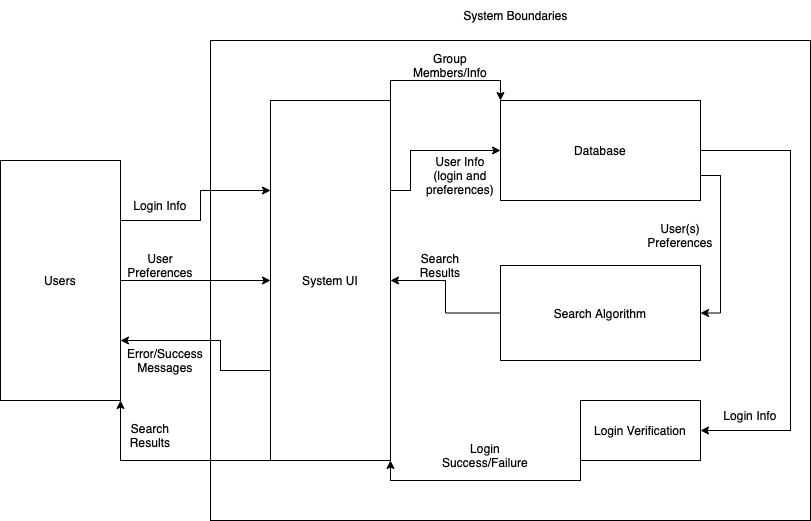
\includegraphics[scale=0.6]{SystemBoundariesDiagram.png}

\subsection{Product Use Case Table}
\begin{tabularx}{\textwidth}{|p{4cm}p{6cm}X|}
	\toprule {\bf Use Case} & {\bf Actors} & {\bf Description}\\
	\hline
	1.0 Create Account & Primary: User & Prompts User for login and password, then stores both in the Database \\
	\hline
	1.1 Verify Login Details \newline (Included in Use Case 1.0) & None & Searches Database for the username and password provided and verifies whether both correspond to the same account \\
	\hline
	1.2 Invalid Login \newline (Extends Use Case 1.0) & None & If the login or password are invalid, shows an error message to the user indicating that the login info was incorrect \\
	\hline
	2.0 Create Preferences & Primary: User & User inputs their movie/show preferences, which the Database stores and connects to their account \\
	\hline
	3.0 Movie Selection & Primary: User & User search for movie/show recommendations based on the input preferences, and the system outputs a list of recommended media based on those preferences \\
	\hline
	3.1 Provide Feedback & Primary: User & Allows User to label a result with "like", "neutral", or "dislike" which will impact what kinds of media the system shows in its results for that User \\
	\hline
	4.0 Create Group & Primary: User/Group Owner \newline Secondary: Other Users & Allows User to create a group and send invites to Other Users \\
	\hline
	5.0 Group Search & Primary: User/Group Owner \newline Secondary: Other Group Users & The Group Owner (user who created the group) will initialte the search for a movie/show, to which the system will respond with a result that takes into account the individual users' preferences \\
	\hline
	\end{tabularx}

\subsection{Individual Product Use Cases}
Please refer to Section 8.2 for individual Use Case descriptions.

\section{Functional Requirements}
\noindent

\subsection{Authentication Requirements} 
\noindent

\textbf{Requirement \#:} 1 \quad \textbf{Requirement Type:} 1 \quad \textbf{Event/Use Case: 1.0}
\medskip
\\\textbf{Description:} The application shall allow the user to signup/login with their email and password
\\\textbf{Rationale:} Allows users to securely sign-in to our application
\\\textbf{Fit Criterion:} Unauthorized users should not be able to access and use the application

\bigskip
\textbf{Requirement \#:} 2 \quad \textbf{Requirement Type:} 1 \quad \textbf{Event/Use Case: 1.0}
\medskip
\\\textbf{Description:} The application shall allow the user to signup/login with an existing Google/Facebook account
\\\textbf{Rationale:} Allows users a convenient method to securely sign-in to the application 
\\\textbf{Fit Criterion:} Unauthorized users should not be able to access and use the application

\bigskip
\textbf{Requirement \#:} 3 \quad \textbf{Requirement Type:} 1 \quad \textbf{Event/Use Case: N/A}
\medskip
\\\textbf{Description:} The application shall allow the user to logout of the application 
\\\textbf{Rationale:} Allows users securely logout of the application 
\\\textbf{Fit Criterion:} User must already be authorized and is logged-in

\subsection{Profile/Group Requirements} 
\noindent

\textbf{Requirement \#:} 4 \quad \textbf{Requirement Type:} 2 \quad \textbf{Event/Use Case: 1.0}
\medskip
\\\textbf{Description:} The application shall allow the user to modify their profile settings (username and password)
\\\textbf{Rationale:} Ensures that users can change their settings if needed
\\\textbf{Fit Criterion:} Username must be unique. Password is required to be longer than 6 characters.

\bigskip
\textbf{Requirement \#:} 5 \quad \textbf{Requirement Type:} 2 \quad \textbf{Event/Use Case: 2.0}
\medskip
\\\textbf{Description:} The application shall allow the user to set their profile preferences 
\\\textbf{Rationale:} Required since the application needs these preferences to efficiently recommend movies/TV shows to the user. The preferences pertain to their favourite genre, movies, TV shows, anime, actors etc.
\\\textbf{Fit Criterion:} The user's input (eg. Movie name) should be valid

\bigskip
\textbf{Requirement \#:} 6 \quad \textbf{Requirement Type:} 2 \quad \textbf{Event/Use Case: 4.0}
\medskip
\\\textbf{Description:} The application shall allow the user to create a group, and specify a group name
\\\textbf{Rationale:} Allows users to create groups so that they can find a recommendation match
\\\textbf{Fit Criterion:} The group name must be unique.

\bigskip
\textbf{Requirement \#:} 7 \quad \textbf{Requirement Type:} 2 \quad \textbf{Event/Use Case: N/A}
\medskip
\\\textbf{Description:} The application shall allow the user to join a group, either through request or invite
\\\textbf{Rationale:} Allows users to join groups so that they can find a recommendation match
\\\textbf{Fit Criterion:} If joining a group through invite, the invite must be valid and specific to the user.

\bigskip
\textbf{Requirement \#:} 8 \quad \textbf{Requirement Type:} 2 \quad \textbf{Event/Use Case: 4.0}
\medskip
\\\textbf{Description:} The application shall allow the user to invite other users based on their username or email
\\\textbf{Rationale:} Allows users to join groups so that they can find a recommendation match
\\\textbf{Fit Criterion:} The username/email invited must be registered as a valid user in our system 

\subsection{Recommendation Requirements} 
\noindent

\textbf{Requirement \#:} 9 \quad \textbf{Requirement Type:} 3 \quad \textbf{Event/Use Case: 3.0}
\medskip
\\\textbf{Description:} The application shall provide an ongoing list of movie/TV show recommendations to the user
\\\textbf{Rationale:} Ensures that the user is consistently getting recommendations to find a possible match
\\\textbf{Fit Criterion:} The recommendation provided must be an existing movie/TV show

\bigskip
\textbf{Requirement \#:} 10 \quad \textbf{Requirement Type:} 3 \quad \textbf{Event/Use Case: 3.1}
\medskip
\\\textbf{Description:} The application shall allow the user to "like", "neutral" or "dislike" each movie/TV show recommendation
\\\textbf{Rationale:} Allows application to continually provide better recommendations and to find a recommendation match
\\\textbf{Fit Criterion:} The user must respond with one of the options: "like", "neutral" or "dislike".

\bigskip
\textbf{Requirement \#:} 11 \quad \textbf{Requirement Type:} 3 \quad \textbf{Event/Use Case: 5.0}
\medskip
\\\textbf{Description:} The application shall notify the group once a recommendation match is found
\\\textbf{Rationale:} The end goal is to provide the group with a recommendation match, so that they can watch that movie/show together.
\\\textbf{Fit Criterion:} The recommendation provided must be an existing movie/TV show and has been approved ("like", "neutral") by the majority of the group. 


\section{Non-Functional Requirements}
a

\subsection{Look and Feel Requirements}


\subsubsection{Appearance Requirements}
The application will start up with a login screen with the options for the username and password of the account, with an "enter" button that does not become available until both the username and password are entered. 
The application will notify the user if an invalid login attempt occured, or if it was successful, bring them into the main page where there will be buttons for logging out, viewing/chaning profile settings, viewing/changing 
media preferences, and creating/joining a group.

\subsubsection{Style Requirements}
The UI will be styled with a consistent and predefined colour pallet, wherein buttons, banners, and other UI elements will have a limited set of different possible colours for the developers to select from. 
The buttons will be placed appropriately, with the size and spacing being optimal for user experience.

\subsection{Usability and Humanity Requirements}
a

\subsubsection{Ease of Use Requirements}
a

\subsubsection{Personalization and Internationalization Requirements}
a

\subsubsection{Learning Requirements}
a

\subsubsection{Understandability and Politeness Requirements}
a

\subsubsection{Accessibility Requirements}
a

\subsubsection{Convenience Requirements}
a

\subsection{Performance Requirements}

\subsubsection{Speed and Latency Requirements}
This application shall immediately (within 1s), by human perception, respond to user input (within 1s after input) The system shall quickly login and logout the user (within 10s).

\subsubsection{Safety-Critical Requirements}
The application shall handle the user's private data with care. 

\subsubsection{Precision or Accuracy Requirements}
The recommendation match provided to the group shall always be the recommendation that is the most approved by the group. The match should have almost zero "dislikes" within the group (cannot always be zero due to certain circumstances). 

\subsubsection{Reliability and Availability Requirements}
The web application shall be available for at least 90\% of the day, given that the servers running the application (on Firebase) are stable.

\subsubsection{Robustness or Fault-Tolerance Requirements}
The application shall always provide users with continual recommendations. The application shall always determine a recommendation match.

\subsubsection{Capacity Requirements}
Each user session within our application is independent of another. Therefore, there is no limit to the number of users who can use our app at once.

\subsubsection{Scalability or Extensibility Requirements}
While scalability is not a major concern, the application should still be scalable in the event that it is needed to do so. 

\subsubsection{Longevity Requirements}
N/A

\subsection{Operational and Environmental Requirements}
a

\subsubsection{Expected Physical Environment}
a

\subsubsection{Wider Environment Requirements}
a

\subsubsection{Requirements for Interfacing with Adjacent Systems}
a

\subsubsection{Productization Requirements}
a

\subsubsection{Release Requirements}
a

\subsubsection{Backwards Compatibility Requirements}
a

\subsection{Maintainability and Support Requirements}

\subsubsection{Maintenance Requirements}
N/A

\subsubsection{Supportability Requirements}
N/A

\subsubsection{Adaptability Requirements}
This product is expected to run on common web browsers (Chrome, Firefox, Edge). It is also expected to run on mobile browsers.

\subsection{Security Requirements}


\subsubsection{Access Requirements}
The application will allow users to access only their own profile settings, while being able to view some of the information of other users.

\subsubsection{Integrity Requirements}
User data will be properly stored and have sufficient protection from corruption.
\subsubsection{Privacy Requirements}
The Developers and those with access to the database will not use or sell user info.

\subsubsection{Audit Requirements}
N/A

\subsubsection{Immunity Requirements}
N/A

\subsection{Cultural Requirements}

\subsubsection{Cultural Requirements}
N/A
\subsection{Compliance Requirements}

\subsubsection{Legal Compliance Requirements}
N/A

\subsubsection{Standards Compliance Requirements}
N/A

\section{Project Issues}


\subsection{Open Issues}

The algorithm to be used that finds appropriate media to recommend to user groups is yet to be determined. While we know the algorithm will be making use of each group members' data as variables, we are deliberating on whether to create one ourselves, or research and use something that already exists.

If we choose to create our own algorithm, we need to have sound reasoning for its logic and structure, and how it makes use of the inputted data.

\subsection{Off-the-Shelf Solutions}

\subsubsection{Ready-Made Products}
N/A

\subsubsection{Reusable Components}
N/A

\subsubsection{Products That Can Be Copied}
There are publicly-known algorithms and methods we can research and implement in our project. We can also consult any open-source applications that make use of recommendation algorithms. It is likely that we will use one or more algorithms that are proven to be successful, and tailor them to our needs, using a combination of pieces as necessary. Creating an algorithm from scratch is a very complex task that is far beyond the scope of this project.

\subsection{New Problems}


\subsubsection{Effects on the Current Environment}
N/A

\subsubsection{Effects on the Installed Systems }
N/A

\subsubsection{Potential User Problems}
N/A

\subsubsection{Limitations in the Anticipated Implementation Environment That May Inhibit the New Product}
N/A

\subsubsection{Follow-Up Problems}
N/A

\subsection{Tasks}

\subsubsection{Project Planning}
N/A

\subsubsection{Planning of the Development Phases}
N/A

\subsection{Migration to the New Product}
N/A

\subsubsection{Requirements for Migration to the New Product}
N/A

\subsubsection{Data That Has to Be Modified or Translated for the New Product}
N/A

\subsection{Risks}

\begin{itemize}
	\item \textbf{Ineffective algorithm:} The main and biggest risk of the project is the algorithm recommending undesirable choices to user groups, which would make our application ineffective at its sole purpose. The probability of this risk actually becoming a problem is very low, as we plan on doing thorough research and analysis of different algorithms to create our customized algorithm using principles that are proven to be successful. Additionally, we will conduct testing using mock data, and make use of the appropriate metrics to determine the effectiveness. Then, we can consider these results to determine if changes should be made - so if our algorithm isn't effective at first, we will eventually reach a final product that is successful.
	\item \textbf{Insecure user login:} With any service that requires users to create an account that has a password for their login, there is the risk of their stored data being compromised. The probability of this risk becoming a problem is low, as we plan on using proper encryption methods for passwords, and implementing Google and Facebook account connection with user authentication.
\end{itemize}


\subsection{Costs}
N/A

\subsection{User Documentation and Training}

\subsubsection{User Documentation Requirements}
N/A

\subsubsection{Training Requirements}
N/A

\subsection{Waiting Room}
N/A

\subsection{Ideas for Solutions}
N/A

\end{document}